\documentclass[12pt,aspectratio=169]{beamer}
% \hypersetup{pdfpagemode=FullScreen}
% \setbeameroption{show notes}
% \setbeameroption{show notes on second screen}

\usepackage{upgreek}
\usefonttheme{professionalfonts}

\usepackage{tikz}

\renewcommand*{\thefootnote}{\fnsymbol{footnote}}

\mode<presentation>
\useoutertheme[subsection=false]{miniframes}

\AtBeginSection[]{
  \begin{frame}
  \centering
  \begin{beamercolorbox}[sep=8pt,center,shadow=true,rounded=true]{title}
    \usebeamerfont{title}\insertsectionhead\par%
  \end{beamercolorbox}
  \end{frame}
}

\title{Accelerating Large-Scale Distributed Neural Network Training with SPMD Parallelism}
\author{\textbf{Shiwei Zhang}\inst{1}\and Lansong Diao\inst{2}\and Chuan Wu\inst{1}\and Siyu Wang\inst{2}\and Wei Lin\inst{2}}
\institute{\inst{1} The University of Hong Kong\and \inst{2} Alibaba Group}
\date{ACM SoCC 2022}

\titlegraphic{\vspace{-1em}
\includegraphics[width=5cm]{hku.png}\hspace*{4.5cm}~%
    \begin{tikzpicture}\node{
\includegraphics[width=4cm]{alibaba.png}};\end{tikzpicture}
}

\begin{document}
    \beamertemplatenavigationsymbolsempty

    \makeatletter
    \def\beamer@andinst{\\[.1em]}
    \makeatother

    \begin{frame}
        \titlepage
    \end{frame}


    \section*{Introduction}

    \begin{frame}
        Deep neural networks (DNN), especially Transformer-based models with \textbf{Mixture-of-Expert (MoE)} layers,
        have become so large that distributed training is necessary.

        \vskip 1em
        Communication overhead is a major problem in distributed DNN training. Using \textbf{TPUs} with fast device-to-device
        links, communication can take up to \textbf{11\%} of training time. On \textbf{GPU clouds} with Ethernet connection,
        communication can take more than \textbf{60\%} of training time.

        \vskip 1em
        We present our system, HiDup, that mitigates the communication overhead by
        \textbf{computation-communication overlapping} and \textbf{overlapping-aware sharding strategy}.

        \note{There are various ways to train a model distributedly and there are many matrue frameworks to choose from.
        However, they all face the same problem: the communication overhead. There must be some kind of communication in
        a distributed system. In DNN training, that's collective communication of tensors.}
    \end{frame}

    \begin{frame}
        \frametitle{Content}

        \begin{itemize}
            \setlength{\itemsep}{.8em}
            \item Background and Motivation
            \item Duplex
            \item Sharding Strategy
            \item Implementation
            \item Evaluation
            \item Conclusion
        \end{itemize}
    \end{frame}


    \section{Background and Motivation}

    \begin{frame}
        \frametitle{Data Parallelism}

        \begin{columns}
            \begin{column}{0.48\textwidth}
                With data parallelism (DP), a minibatch of training data is split along the batch size dimension and
                each worker processes a slice independently. \texttt{All-Reduce} is used to synchonize the grandients
                at the end of each iteration.
                \vskip 1em
                \centering
                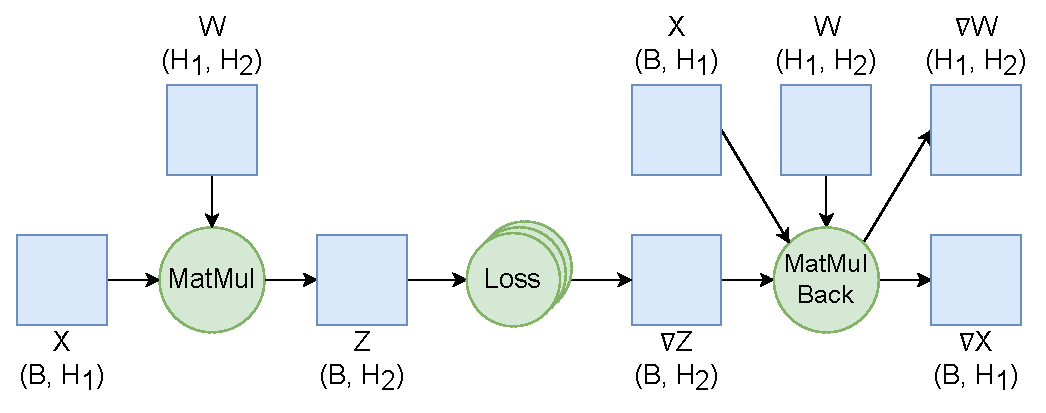
\includegraphics[width=.85\textwidth]{toy_example_single.pdf}
            \end{column}
            \begin{column}{0.55\textwidth}
                \centering
                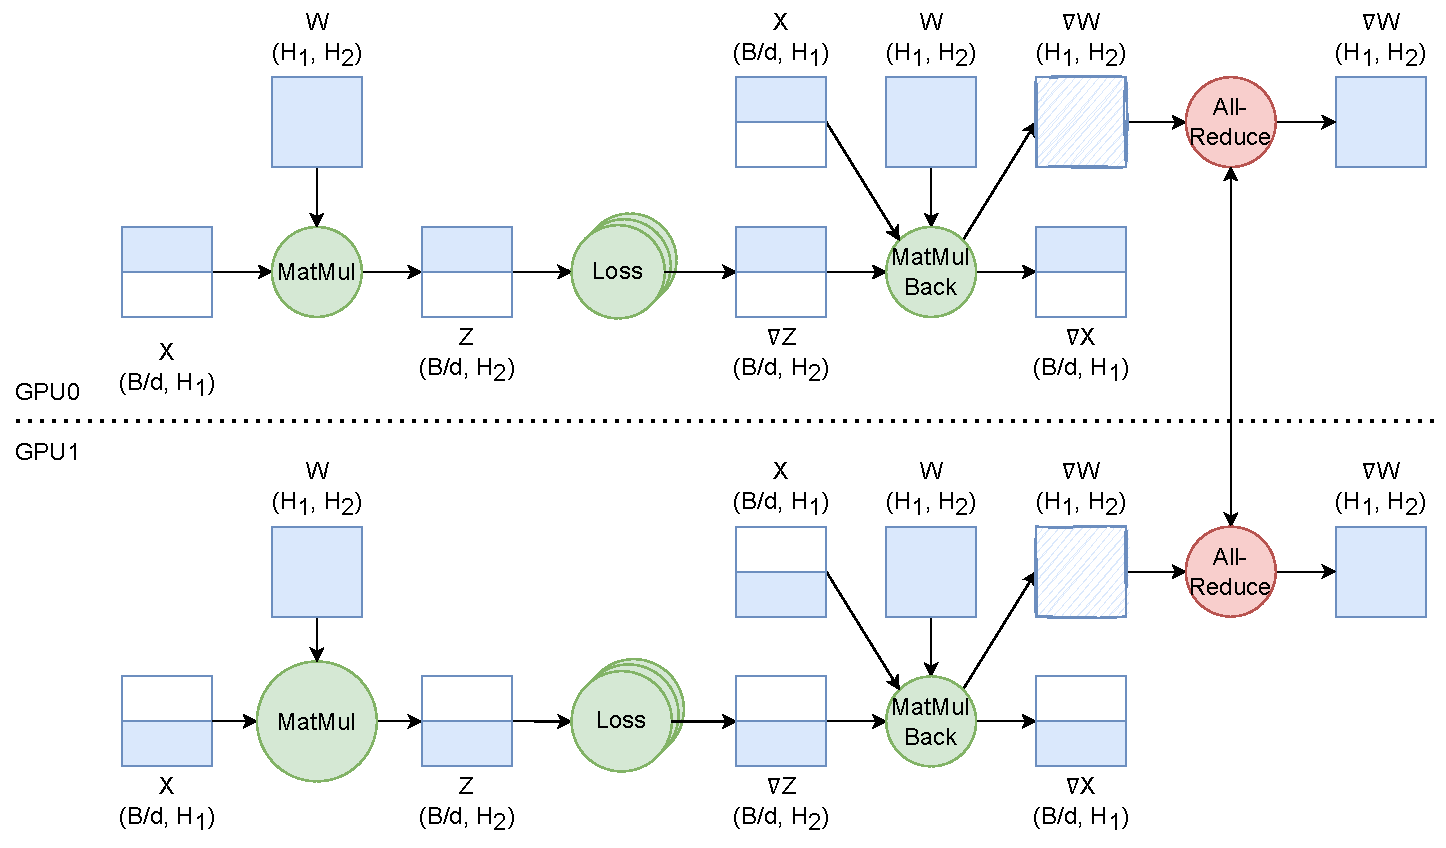
\includegraphics[width=\textwidth]{toy_example_dp.pdf}
            \end{column}
        \end{columns}

    \end{frame}

    \begin{frame}
        \frametitle{SPMD Parallelism}

        DP does not support models that exceed the memory of a single device. SPMD parallelism is a more general method
        that allows sharding along any dimension of any tensor. Collective communication is needed when the sharding
        methods of two tensors are incompatible.

        \vskip 1em
        \centering
        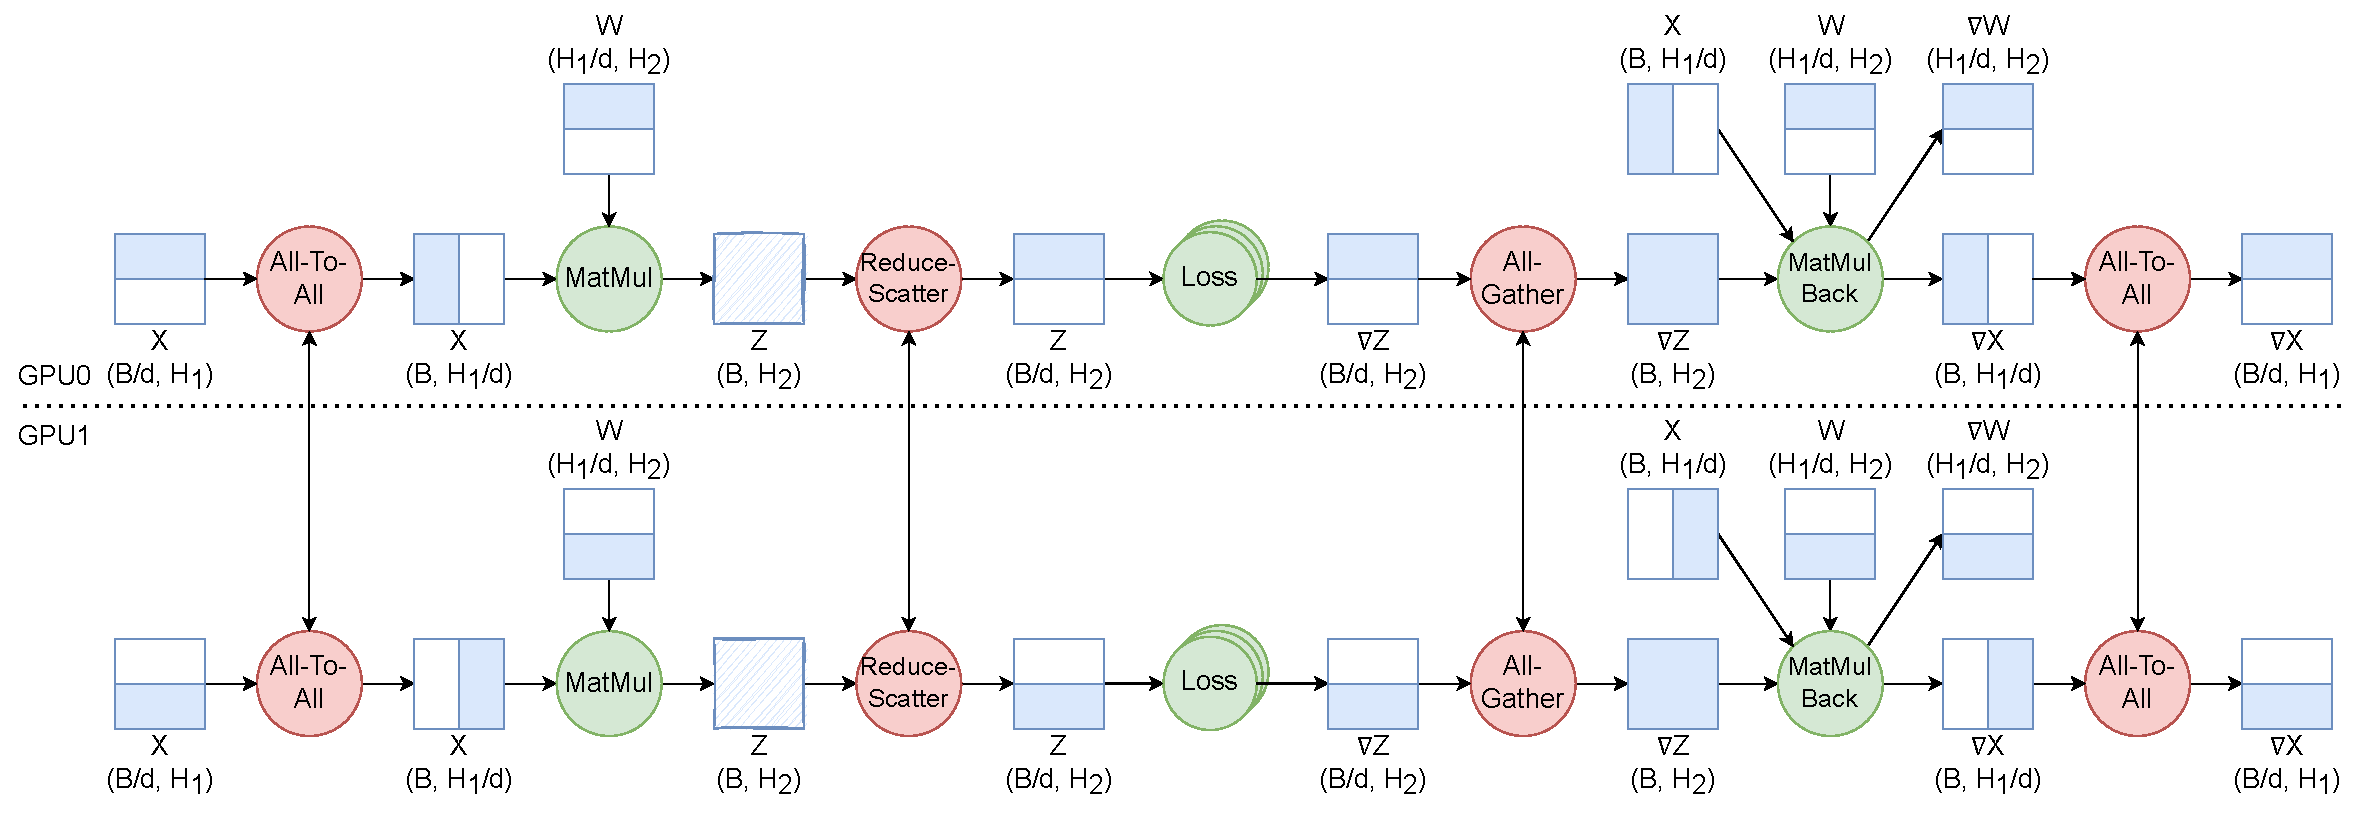
\includegraphics[width=.85\textwidth]{toy_example_mp.pdf}
    \end{frame}


    \begin{frame}
        \frametitle{SPMD Parallelism Examples}

        \begin{columns}
            \begin{column}{0.5\textwidth}
                \centering
                \includegraphics[page=4,trim=10.9cm 17.5cm 1.9cm 2.2cm,clip,scale=0.75]{megatron.pdf}
                \hbox{\tiny Source: Shoeybi, M., et al.~``Megatron-LM'' (2019).}
            \end{column}
            \begin{column}{0.5\textwidth}
                \centering
                \vskip -1.5em
                \includegraphics[page=5,trim=10.5cm 16.8cm 4cm 3cm,clip,scale=0.83]{GShard.pdf}
                \hbox{\tiny Source: Lepikhin, D., et al.~``GShard'' (2020).}
            \end{column}
        \end{columns}
    \end{frame}


    \section*{Duplex}

    \begin{frame}
        \centering
        \begin{beamercolorbox}[sep=8pt,center,shadow=true,rounded=true]{title}
          \usebeamerfont{title}Duplex: Enable Computation-Communication Overlapping with SPMD Parallelism\par%
        \end{beamercolorbox}
    \end{frame}

    \begin{frame}
        \frametitle{Duplex}

        \begin{columns}
            \begin{column}{0.54\textwidth}
                Inspired by gradient accumulation, we split the input data on each worker into two microbatches
                \textbf{after applying SPMD parallelism}, and scheduling the two microbatches into a pipeline such that
                the computation of one microbatch overlaps with the communication of the other microbatch.
            \end{column}
            \begin{column}{0.5\textwidth}
                \centering
                \vskip -1em
                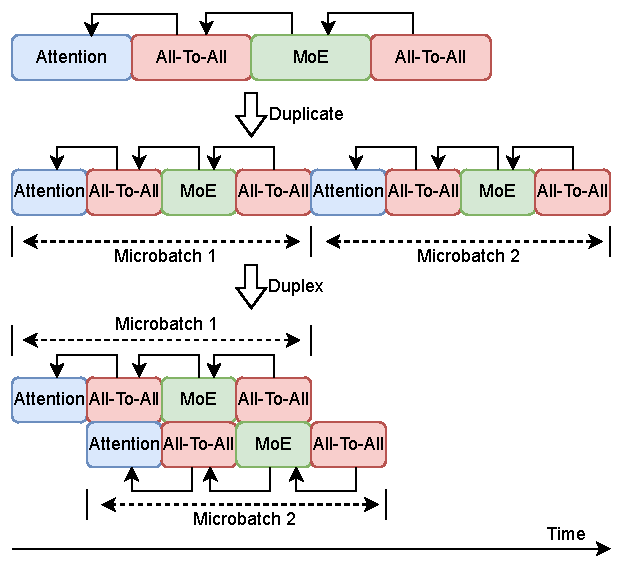
\includegraphics[width=.9\textwidth]{duplex.pdf}
            \end{column}
        \end{columns}
    \end{frame}

    \begin{frame}
        \frametitle{Duplex Example}

        \centering
        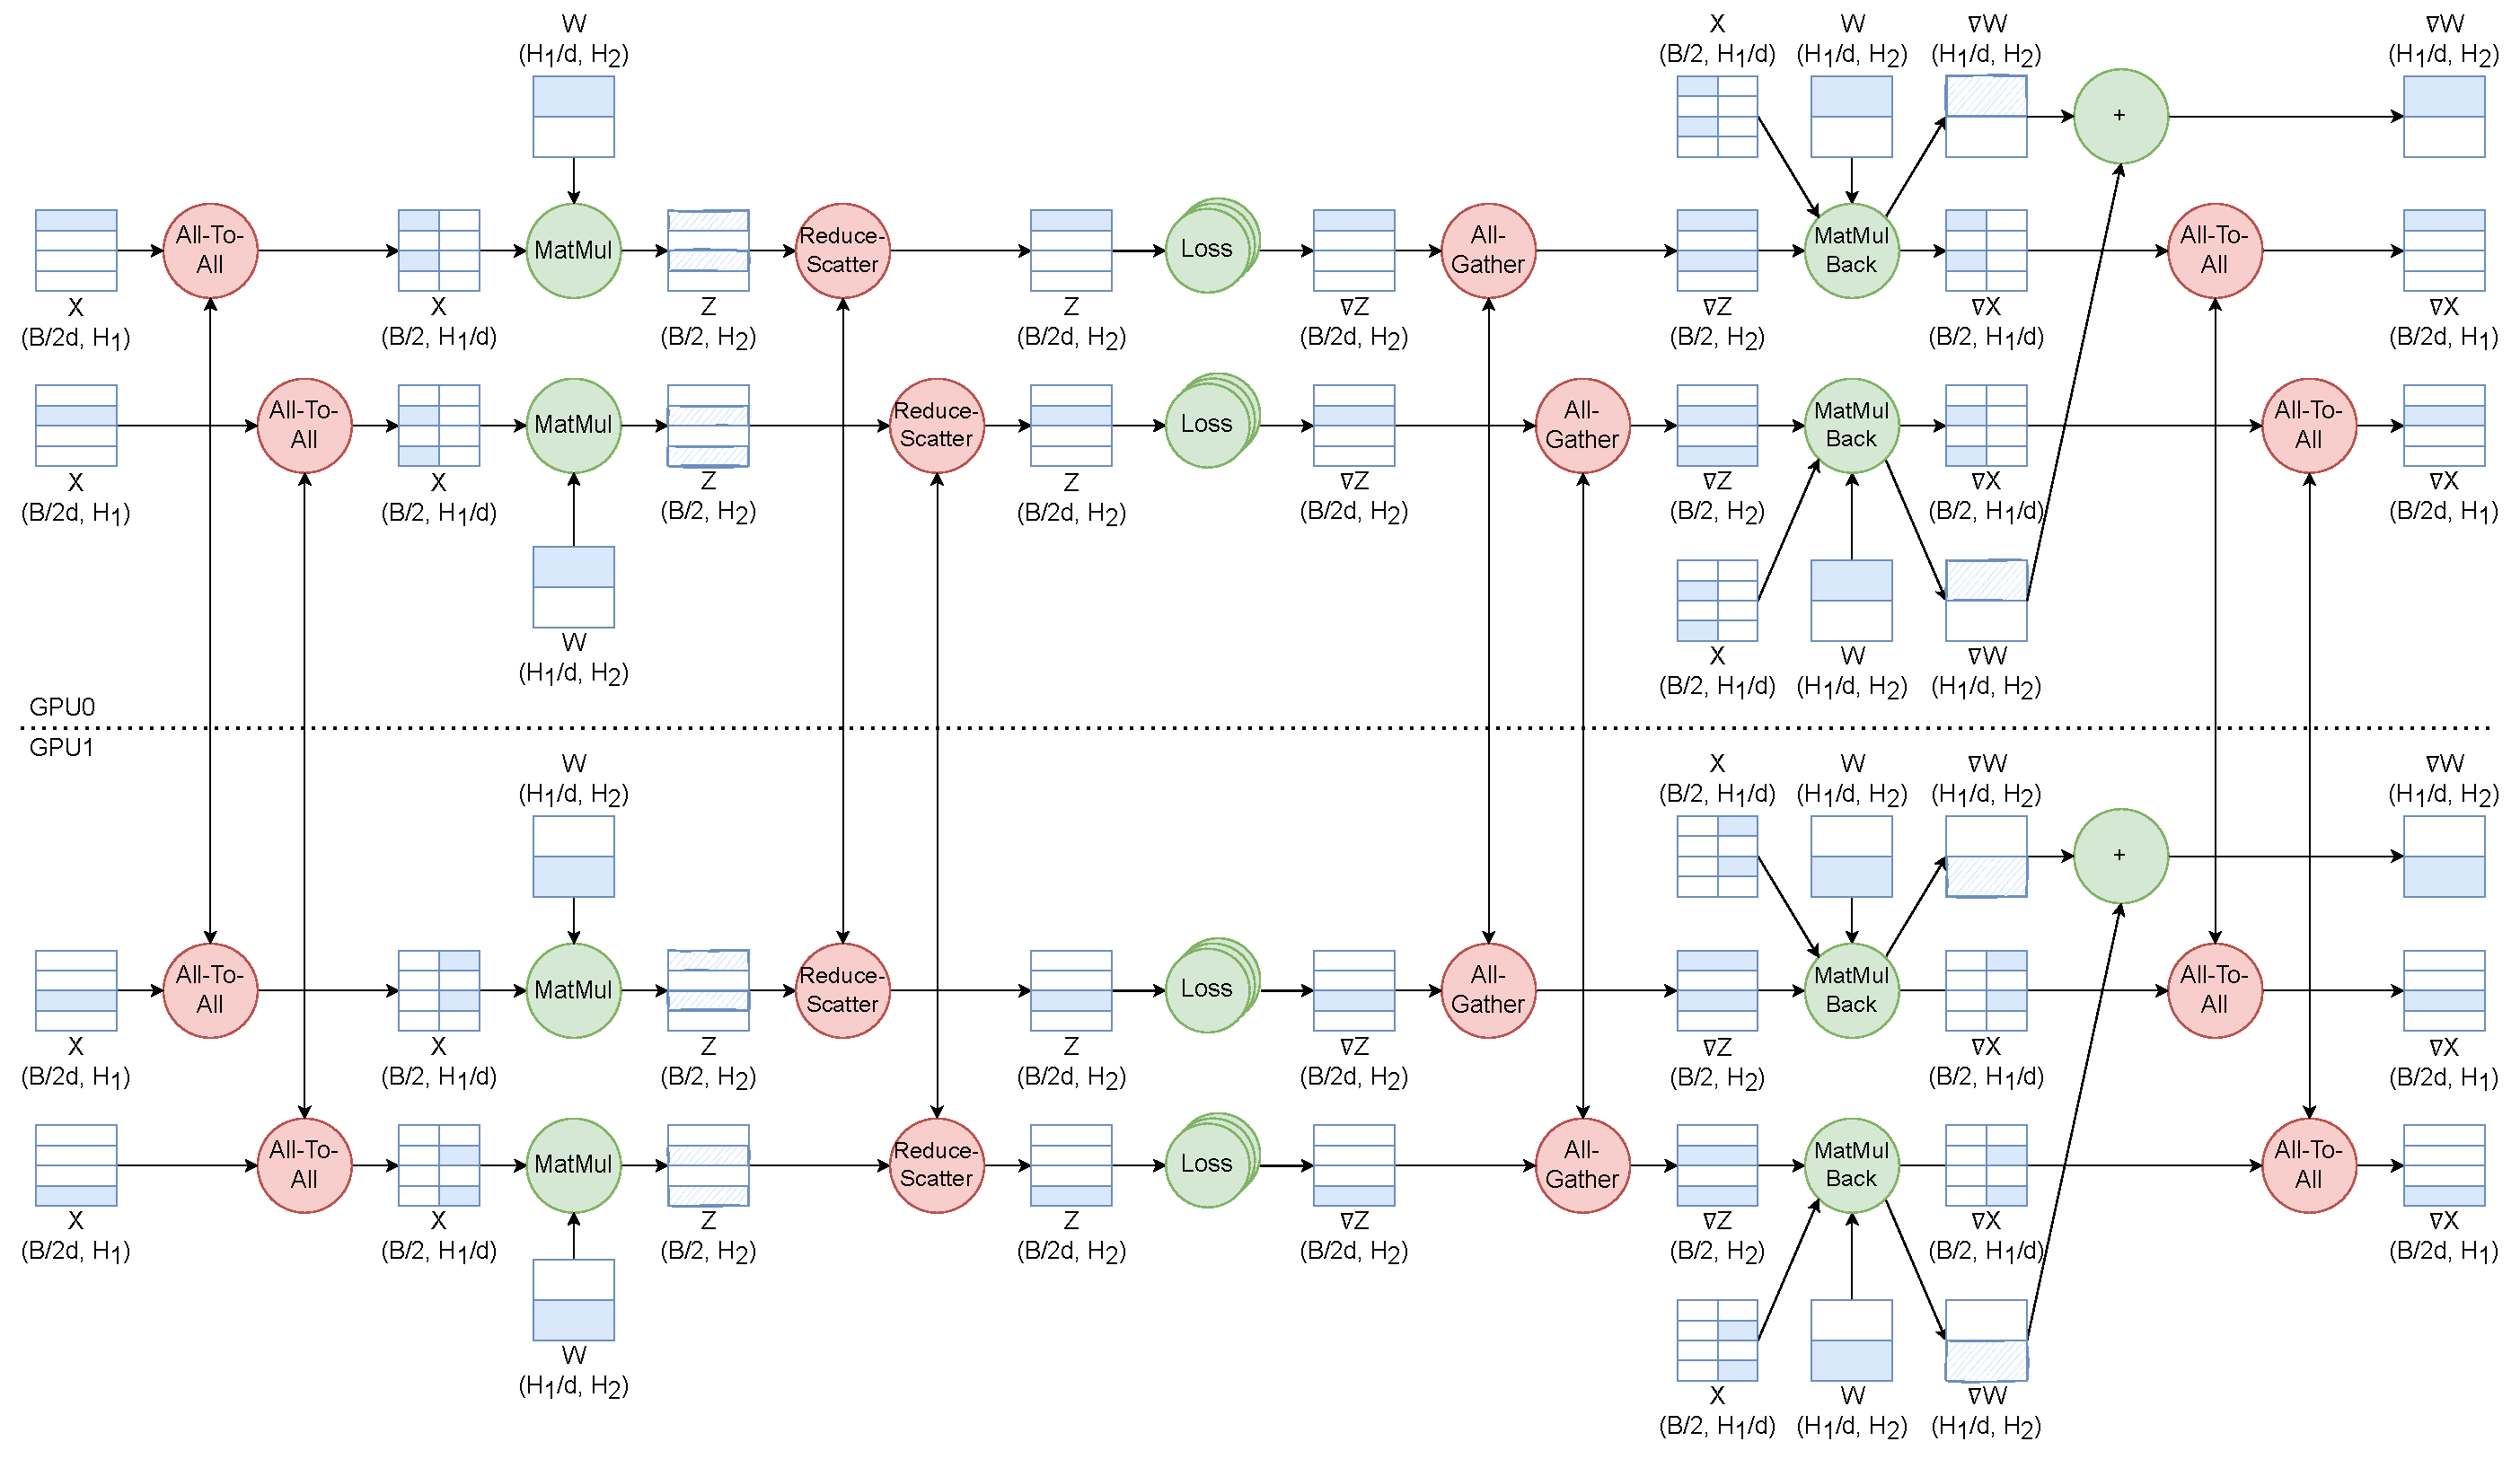
\includegraphics[width=.9\textwidth]{toy_example_duplex.pdf}
    \end{frame}

    \begin{frame}
        \frametitle{Duplex}

        \begin{itemize}
            \setlength{\itemsep}{.8em}
            \item \textbf{Accuracy}: Only floating-point arithmetic errors.
            \item \textbf{Memory Usage}: No increase.
            \item \textbf{GPU Utilization}: Slightly reduced due to smaller tensor sizes.
            \item \textbf{Overheads}: CUDA synchonization, gradient aggregation, memory bus contention, interference between computation and communication.
            \item \textbf{Speed-up}: Up to 100\% in ideal case.
        \end{itemize}
    \end{frame}


    \section*{Sharding Strategy}

    \begin{frame}
        \centering
        \begin{beamercolorbox}[sep=8pt,center,shadow=true,rounded=true]{title}
          \usebeamerfont{title}Duplex-aware Sharding Strategy\par%
        \end{beamercolorbox}
    \end{frame}

    \begin{frame}
        \frametitle{Motivation}

        With the fast emergence of new DNN models, manually designing SPMD strategies for each model is manpower
        intensive and time-consuming. Further, the strategy may not always be optimal on different clusters.

        \vskip 1em
        Existing studies search for sharding strategy that \textbf{minimizes communication volume}. This strategy
        may not be optimal when used together with Duplex.
    \end{frame}

    \begin{frame}
        \frametitle{Sharding Strategy}

        \begin{itemize}
            \setlength{\itemsep}{.8em}
            \item \textbf{Objective}: Find the sharding methods for all operators that minimizes the training time with computation-communication overlapping.
            \item \textbf{Basic Idea}: Using dynamic programming to incrementally search for the best strategies of a subgraph.
            \item \textbf{Challenge}: The best strategy of a subgraph may not be optimal for the complete graph due to computation-communication overlapping.
            \item \textbf{Solution}: We propose a stage-based cost model and track two costs associated with a search state.
        \end{itemize}
    \end{frame}

    \begin{frame}
        \frametitle{Sharding Strategy}

        \begin{columns}
            \begin{column}{0.5\textwidth}
                {
                \centering
                \includegraphics[page=8,trim=2.2cm 20cm 11.2cm 2.8cm,clip,scale=0.84]{paper.pdf}
                }

                More details in the paper.
            \end{column}
            \begin{column}{0.54\textwidth}
                \centering
                \vskip -2em
                \includegraphics[page=8,trim=11cm 17cm 2.2cm 2.8cm,clip,scale=0.8]{paper.pdf}
            \end{column}
        \end{columns}
    \end{frame}

    \section{Implementation}

    \begin{frame}
        \frametitle{Implementation}

        We implement HiDup as a graph transformation module on PyTorch. It takes as input a single-card model (as
        PyTorch fx graph) and the cluster specification, producing a modified graph that runs on all workers.

        \vskip 1em
        \centering
        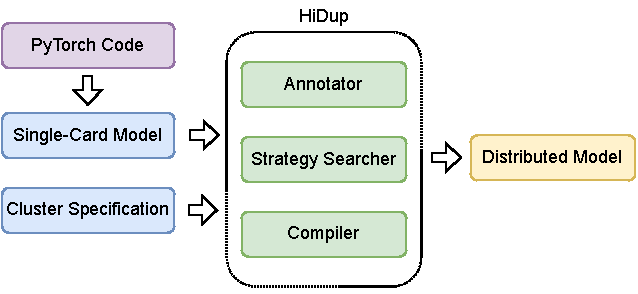
\includegraphics[width=.5\textwidth]{arch.pdf}
    \end{frame}

    \begin{frame}
        \frametitle{Implementation}

        \begin{itemize}
            \setlength{\itemsep}{.8em}
            \item \textbf{Annotator}: Label the possible sharding methods for each operator, infer the tensor sizes, and estimate the FLOPs.
            \item \textbf{Strategy Searcher}: Take annotated graph as input and search for the optimal sharding strategy.
            \item \textbf{Compiler}: Modify the graph according to the strategy and applies Duplex.
        \end{itemize}

        \note{The annotator encodes the domain knowledge, the other two components are generic. To add support for a new operator, only the annotator needs to be modified.}
    \end{frame}

    \section{Evaluation}

    \begin{frame}
        \frametitle{Experimental Setup}

        \begin{itemize}
            \setlength{\itemsep}{.8em}
            \item \textbf{Testbed}: 8 machines on public cloud, each with 8 V100 GPUs and NVLink, connected by 10Gbps network.
            \item \textbf{Benchmarks}: BERT (language modeling) and ViT (image classification), with two variants of MoE layers, SGMoE and Switch.
            \item \textbf{Baselines}: DeepSpeed, FastMoE, PyTorch DDP, and Horovod.
        \end{itemize}
    \end{frame}

    \begin{frame}
        \frametitle{Per-iteration training time}

        \includegraphics[page=10,trim=2.2cm 20.5cm 2.2cm 2.6cm,clip,scale=0.8]{paper.pdf}

        \vskip 1em
        HiDup outperforms baselines when scaling up, because the collective communication becomes slower with more cards
        and HiDup can mitigate the increased communication overhead with our Duplex design.
    \end{frame}

    \begin{frame}
        \frametitle{Single Machine Performance}

        \includegraphics[page=10,trim=2.2cm 15cm 2.2cm 8.1cm,clip,scale=0.8]{paper.pdf}

        \vskip .5em
        Pure-DP methods perform well with high bandwidth. HiDup automatically identifies similar strategies and achieves
        comparable performance despite of the additional overheads introduced by our Duplex design.
    \end{frame}

    \begin{frame}
        \frametitle{Per-iteraion time breakdown}

        \includegraphics[page=13,trim=2.2cm 21cm 2.2cm 3.5cm,clip,scale=0.81]{paper.pdf}

        HiDup's total time is similar to the baselines, but it achieves shorter wall time by overlapping computation
        and communication.
    \end{frame}

    \begin{frame}
        \frametitle{SPMD Strategy}

        \begin{columns}
            \begin{column}{0.48\textwidth}
                HiDup generates different strategies for the same model on different clusters.

                \vskip 1em
                It automatically identifies expert-designed strategies for common models.
            \end{column}
            \begin{column}{0.55\textwidth}
                \centering
                \vskip -2em
                \includegraphics[page=13,trim=2cm 12.9cm 11.2cm 6.8cm,clip,scale=0.84]{paper.pdf}
            \end{column}
        \end{columns}
    \end{frame}


    \section{Conclusion}

    \begin{frame}
        \frametitle{Conclusion}

        \begin{itemize}
            \setlength{\itemsep}{.8em}
            \item We propose Duplex that enables computation-communication overlapping with SPMD parallelism.
            \item We design a Duplex-aware sharding strategy search algorithm.
            \item We explore graph transformation on PyTorch and implement HiDup based on PyTorch fx.
        \end{itemize}
    \end{frame}

    \appendix

    \begin{frame}
        \vskip 1em

        \vskip 1em
        \centering
        {\huge Thank you!}
        \vskip 1em
        Email: swzhang@cs.hku.hk

    \end{frame}
\end{document}
